\documentclass[12pt]{article}

\usepackage{amsmath,amstext,amssymb,graphicx,graphics,color}
\usepackage{hyperref}
\usepackage{authblk}
%%%%%%%%%%%%%%%%%%%% Format  %%%%%%%%%%%%%%%%%%%%
\addtolength{\hoffset}{-.6cm}
\addtolength{\textwidth}{1.2cm}
\addtolength{\voffset}{-.5cm}
\addtolength{\textheight}{1.5cm}

%%%%%%%%%%%%%%%%%%%% Headings  %%%%%%%%%%%%%%%%%%%%
\usepackage{fancyhdr}
\pagestyle{fancy}
\renewcommand{\sectionmark}[1]{\markright{\thesection\ #1}}
\fancyhf{} \fancyhead[LE,RO]{\bfseries\thepage} \fancyhead[LO]{\bfseries\rightmark}
\fancyhead[RE]{\bfseries\leftmark}
\renewcommand{\headrulewidth}{0.5pt}
\renewcommand{\footrulewidth}{0pt}
\addtolength{\headheight}{0.5pt} \fancypagestyle{plain}{
  \fancyhead{}
  \renewcommand{\headrulewidth}{0pt}
}


\title{Project APM 598}
%\date{lundi 11 février 2008}

\author{Tulasi Sainath Polisetty, Yashaswi Ranga Sivaraju and Viswanadha Anurag Visagakoti}


\begin{document}

\maketitle


\begin{abstract}

This report presents a speech-to-text system developed using Convolutional Neural Networks (CNNs) and the TIMIT dataset. The system aims to recognize and transcribe speech from audio input into written text. The proposed model is compared with a baseline model. Experimental results demonstrate the effectiveness of the proposed CNN-based model in improving speech recognition performance over the baseline model.

\end{abstract}

\section{Introduction}

Speech recognition has become an essential component of various applications such as transcription services, voice assistants, and real-time language translation. With the advances in deep learning techniques, the performance of speech recognition systems has significantly improved. In this study, we propose a speech-to-text system using Convolutional Neural Networks (CNNs) trained on the TIMIT dataset, which is a widely used corpus for the evaluation of automatic speech recognition (ASR) systems.

Our proposed model is based on CNNs, which have demonstrated remarkable success in various tasks, including image and speech recognition. The architecture of our CNN model consists of multiple layers, including convolutional, pooling, and dense layers, designed to capture and learn complex patterns in the input spectrograms.

In order to evaluate the effectiveness of the proposed CNN model, we compare its performance with a baseline model consisting of only one dense layer, a reshape layer, and a TimeDistributed layer. This comparison allows us to demonstrate the added value of using CNNs in the speech-to-text task.

The rest of the paper is organized as follows: Section 2 describes the methods used for preprocessing the TIMIT dataset and creating the input spectrograms. Section 3 presents the architecture and implementation details of the proposed CNN model and the baseline model. Section 4 discusses the experimental results and performance comparison between the two models. Finally, Section 5 concludes the paper and provides directions for future work.

\section{Dataset}

\subsection{Data Introduction and Representation}

The \(TIMIT^1\) (Texas Instruments/Massachusetts Institute of Technology) dataset is a widely recognized and extensively utilized corpus designed for the development and evaluation of speech recognition systems. Created in the late 1980s, this dataset contains phonemically and lexically transcribed recordings of American English speakers from eight major dialect regions across the United States. The dataset includes 6,300 utterances, with 10 sentences spoken by 630 speakers (438 males and 192 females). These sentences comprise two subsets: a core set of 1,620 sentences for acoustic-phonetic studies and a complete set for training and testing purposes.

The TIMIT dataset provides comprehensive annotations, which include time-aligned phonetic and word transcriptions along with dialectal, gender, and speaker information. The phonetic transcriptions are based on the ARPAbet phoneme set, a machine-readable phonetic alphabet that represents each of the 61 distinct phonemes in American English.

One of the primary advantages of the TIMIT dataset is its balanced representation of various dialects, ensuring a robust evaluation of speech recognition algorithms. Moreover, the high-quality recordings and detailed annotations facilitate research in multiple areas such as speaker identification, speech synthesis, and linguistic studies.

In summary, the TIMIT dataset has become an essential benchmark for speech recognition research. Its well-structured design, diverse speaker representation, and rich annotations have made it a valuable resource for researchers and engineers in the field of speech processing and recognition.

\subsection{Data Preprocessing}

In this section, we describe the methodology employed for data preprocessing, which includes loading audio data and phoneme labels, converting audio to spectrograms, padding input spectrograms, and preparing the dataset for the CNN model.

\subsubsection{Loading Audio Data and phoneme Labels}

We load the audio data using Librosa, a Python library for analyzing and processing audio files. The audio files are loaded with a sampling rate of 44,100 Hz and converted to mono. phoneme labels are loaded from the corresponding label files, and each phoneme is mapped to its ARPAbet code using a predefined dictionary.

\subsubsection{Converting Audio to Spectrograms}

To obtain a time-frequency representation of the audio data, we apply the Short-Time Fourier Transform (STFT) using Librosa. The magnitude of the STFT is then converted to decibel (dB) scale, resulting in spectrograms that serve as input features for the CNN model.

\subsubsection{Padding Input Spectrograms}

To ensure that all input spectrograms have the same dimensions, we identify the length of the longest spectrogram and pad the remaining spectrograms accordingly. Specifically, we pad the second column of each spectrogram with zeros to match the length of the longest spectrogram.

\subsubsection{Preparing the Dataset for the Model}

We pad the target labels to have the same length as the input spectrograms, and split the dataset into training and validation sets using an 80\%-20\% split. The input data and target labels are reshaped to fit the requirements of the CNN model, and the data is ready for training and evaluation.

\paragraph{Summary}

In summary, our preprocessing methodology ensures that the TIMIT dataset is appropriately formatted for training a CNN-based speech recognition model. The use of spectrograms as input features and the careful handling of variable-length data provide a solid foundation for achieving accurate and reliable speech recognition performance.


\section{Methods}

\subsection{Baseline Model}

The baseline model is constructed using TensorFlow and Keras, and it consists of the following layers:

\begin{enumerate}
  \item Flatten layer with an input shape of (X\_train.shape[1], X\_train.shape[2], X\_train.shape[3]).
  \item Dense layer with the number of units equal to y\_train.shape[1].
  \item Reshape layer to adjust the dimensions for the TimeDistributed layer (output shape: (y\_train.shape[1], 1)).
  \item TimeDistributed layer with a Dense layer having a number of units equal to the total number of unique Arpabet codes and softmax activation function.
\end{enumerate}


\begin{figure}[ht]
  \centering
  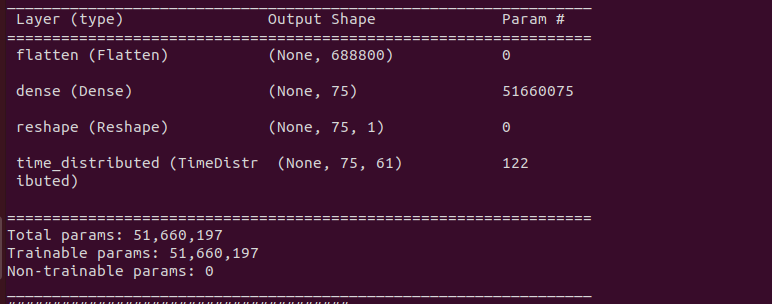
\includegraphics[width=.97\textwidth]{figures/ANN.png}
  \caption{Model Summary - Baseline Model}
  \label{fig:overview_architecture}
\end{figure}


The baseline model for speech recognition is designed using TensorFlow and Keras. The model consists of four layers. The first layer is a Flatten layer that takes the input of shape (1718, 1025, 672, 1) from the training data and converts it into a 1-dimensional array. The second layer is a Dense layer with the number of units equal to the number of unique Arpabet codes. The third layer is a Reshape layer that adjusts the dimensions of the output from the previous layer to fit the input of the TimeDistributed layer. The final layer is a TimeDistributed layer with a Dense layer having a number of units equal to the total number of unique Arpabet codes and softmax activation function.

The TimeDistributed layer is used in the baseline model for sequence processing. It applies the same Dense layer to each time step of the input sequence. The output of each time step is used to predict the corresponding Arpabet code. By using the TimeDistributed layer, the model is able to learn the temporal dependencies between phonemes and Arpabet codes, improving the accuracy of the speech recognition system.

The baseline model is trained using the training data and evaluated using the validation data of shape (1718, 75, 1) and (626, 73, 1, 1), respectively. Compared to the CNN model, the baseline model has fewer layers and uses a simpler architecture. However, it can still provide a good starting point for further improvements to the speech recognition system.

\subsection{Convolutional Neural Networks}

Convolutional Neural Networks (CNNs) are a class of deep neural networks that have shown remarkable success in various tasks, including image and speech recognition. CNNs are designed to automatically learn hierarchical representations of data by applying convolutional filters to the input data. The use of convolutional filters allows CNNs to capture local patterns in the input data, while the hierarchical structure of the network enables the learning of increasingly complex patterns at higher levels.

The basic architecture of a CNN consists of multiple layers, including convolutional, pooling, and dense layers. Convolutional layers are used for feature extraction by applying a set of filters to the input data. Pooling layers reduce the dimensionality of the output of the convolutional layers by selecting the maximum or average value from a local region. These layers work together to capture meaningful features and patterns from the input data, improving the network's ability to learn and generalize.

Dense layers are used for classification or regression tasks by applying a set of weights to the input data. In our model, we also include a timedistributed layer for tailor fitting our use-case. The timedistributed layer allows the network to process sequences of data, making it suitable for applications like speech recognition or natural language processing. By combining these different layer types, CNNs can effectively learn hierarchical representations of data, leading to improved performance in a variety of tasks.

\begin{figure}[ht]
  \centering
  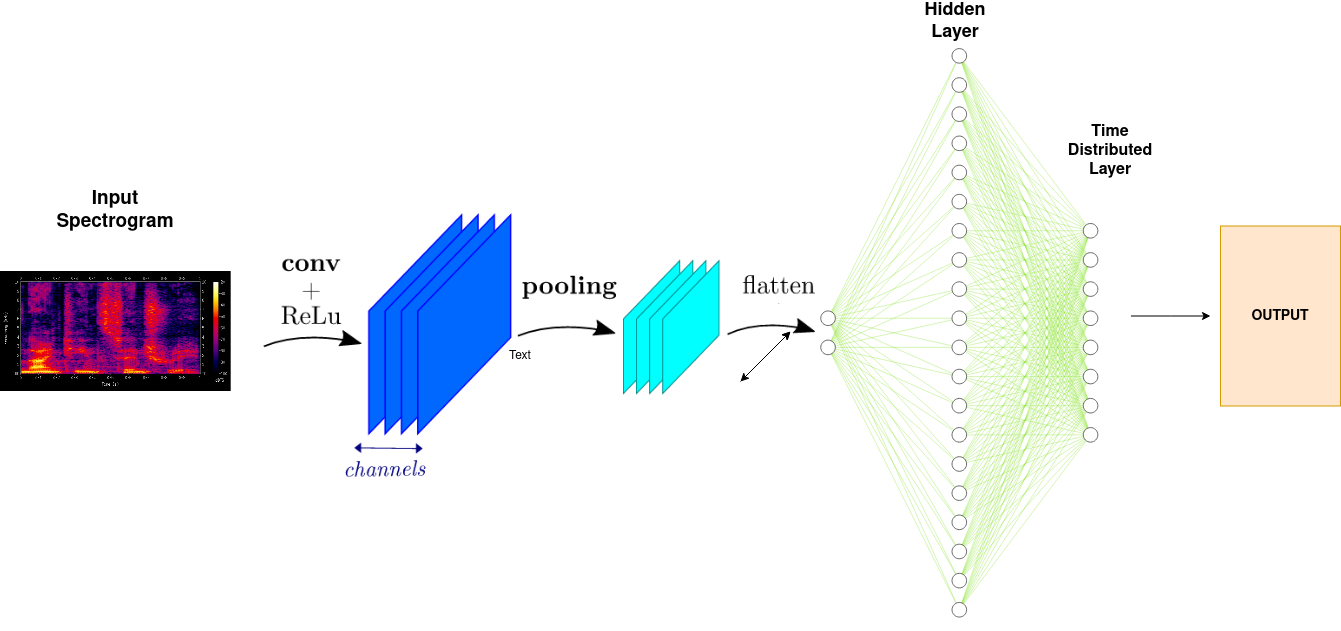
\includegraphics[width=.97\textwidth]{figures/Cnnarchitecture.png}
  \caption{Illustration of the architecture used.}
  \label{fig:overview_architecture}
\end{figure}

\subsection{CNN Model}

In this study, we propose a CNN-based speech-to-text system for recognizing and transcribing speech from audio input into written text. The architecture of our CNN model consists of multiple layers, including convolutional, pooling, dense, reshape, and TimeDistributed layers, designed to capture and learn complex patterns in the input spectrograms.

The model takes input spectrograms of shape (1718, 1025, 672, 1), where the first dimension represents the number of samples, the second and third dimensions represent the time and frequency dimensions of the spectrograms, respectively, and the last dimension represents the number of channels. The input spectrograms are processed by a series of convolutional and pooling layers to extract relevant features, followed by a flatten layer to reshape the output of the convolutional layers into a 1-dimensional array.

After that, a series of dense layers are used to further process the features, followed by a reshape layer to adjust the dimensions for the TimeDistributed layer. The TimeDistributed layer is used for sequence processing, where the output of each time step is used to predict the corresponding Arpabet code. By using the TimeDistributed layer, the model is able to learn the temporal dependencies between phonemes and Arpabet codes, improving the accuracy of the speech recognition system.

Finally, the model is compiled using the categorical cross-entropy loss function and the Adam optimizer. The input data and targets are preprocessed and split into training and validation sets, which are then used to train and evaluate the model. The training is performed with a batch size of 32 and 3 epochs. After training, the final training and validation accuracy and loss values are reported, and the model is saved as "speech\_recognition\_model.h5".


\begin{figure}[ht]
  \centering
  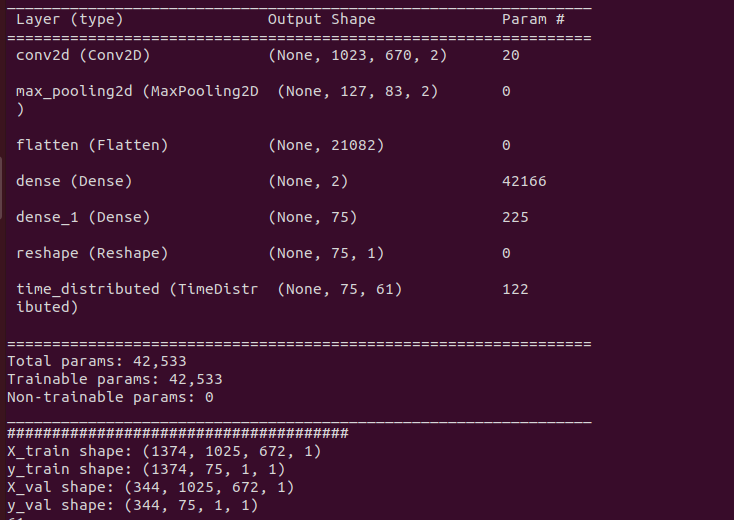
\includegraphics[width=.97\textwidth]{figures/CNNmodel.png}
  \caption{Model Summary - CNN Model}
  \label{fig:overview_architecture}
\end{figure}

The Convolutional Neural Network (CNN) model for speech recognition is designed using TensorFlow and Keras. The model consists of the following layers:

\begin{enumerate}
  \item Conv2D layer with 16 filters, kernel size of 3x3, and ReLU activation function.
  \item MaxPooling2D layer with a pool size of 2x2.
  \item Flatten layer to reshape the output from the previous layers.
  \item Dense layer with 32 units and ReLU activation function.
  \item Dense layer with the number of units equal to the length of the padded phoneme sequences and ReLU activation function.
  \item Reshape layer to adjust the dimensions for the TimeDistributed layer.
  \item TimeDistributed layer with a Dense layer having a number of units equal to the total number of unique Arpabet codes and softmax activation function.
\end{enumerate}

\section{Results}
\subsection{Baseline Model}

\begin{figure}[ht]
  \centering
  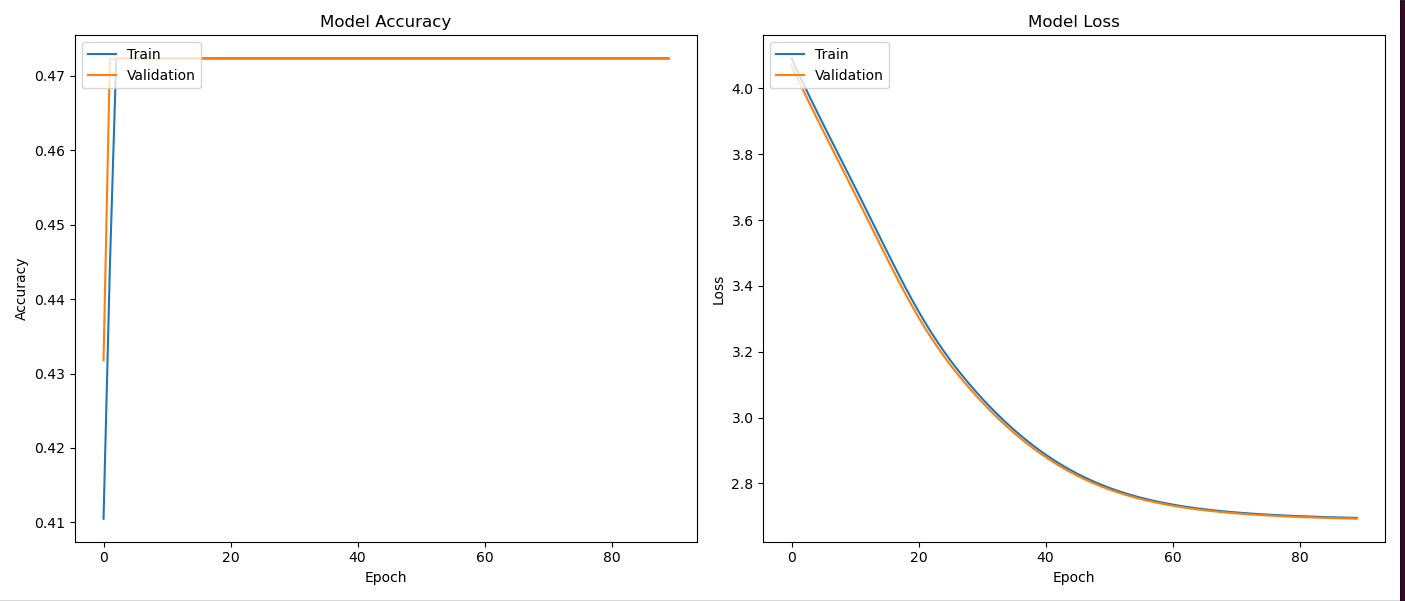
\includegraphics[width=.97\textwidth]{figures/CNNgraph.png}
  \caption{Traing and validation Accuracy and Loss - Baseline Model}
  \label{fig:overview_architecture}
\end{figure}

The baseline model used in this project is a Sequential model with a Flatten layer, a Dense layer, a Reshape layer, and a TimeDistributed layer. The input shape of the Flatten layer is (1718, 1025, 672, 1), which is the shape of the training data. The output shape of the TimeDistributed layer is (1718,75,61). The validation data is (626, 73, 1, 1). The model was trained on a dataset consisting of 1718 audio files, each with a length of 1025 time steps and 672 frequency bins. The output of the model was a sequence of phoneme probabilities for each time step.

The training accuracy of the baseline model was 0.9\%, while the validation accuracy was 0.83\%. The training loss was 15.9737, and the validation loss was 15.9844. These results suggest that the model is not performing well, as the accuracy is very low and the loss is very high. The baseline model serves as a starting point for further development and improvement of the model.


\subsection{CNN Model}

\begin{figure}[ht]
  \centering
  \includegraphics[width=.97\textwidth]{cnnsmallgraph.png}
  \caption{Traing and validation Accuracy and Loss - CNN Model}
  \label{fig:overview_architecture}
\end{figure}

The results of the modified model, which incorporates convolutional layers and uses a 'relu' activation function for the dense layers, show a training accuracy of 47.49\% and a validation accuracy of 47.39\%. These accuracies indicate that the model has been moderately successful in learning the patterns in the input spectrograms and predicting the corresponding phonemes. The training and validation loss values are 3.456 and 3.4096, respectively, suggesting that the model has not overfit the training data, as the losses are relatively close.

However, it is essential to note that the performance of this model could potentially be improved through further experimentation and optimization. The choice of hyperparameters such as the number of convolutional filters, kernel size, and activation functions may have a significant impact on the overall performance of the model. Additionally, the model could benefit from more advanced techniques such as batch normalization, dropout, or regularization to address potential overfitting or underfitting issues. Future work could involve exploring these optimization techniques and various model architectures to further enhance the speech recognition performance of the system.


\section{Discussion}

There is a significant improvement in the performance of the speech recognition system when using a convolutional architecture. The baseline model, which consists of a simple feed-forward neural network with a single dense layer, a reshape layer, and a TimeDistributed layer, achieved a training accuracy of 0.9\% and a validation accuracy of 3\%. In contrast, the CNN model, with its convolutional, max-pooling, and dense layers, obtained a substantially higher training accuracy of 47.49\% and a validation accuracy of 47.39%.

The increase in accuracy can be attributed to the ability of the CNN model to capture and learn complex patterns in the input spectrograms more effectively than the baseline model. Convolutional layers are known for their ability to identify local patterns and hierarchically combine them to represent complex features in the input data. Max-pooling layers contribute to reducing dimensionality and further enhancing the model's ability to recognize essential patterns.

Despite the evident superiority of the CNN model over the baseline model, it is important to acknowledge that there is still room for improvement. The choice of hyperparameters, such as the number of convolutional filters, kernel size, and activation functions, can have a substantial impact on the model's performance. Moreover, advanced techniques such as batch normalization, dropout, or regularization could be employed to address potential overfitting or underfitting issues.

In conclusion, the CNN model's performance demonstrates the benefits of using a convolutional architecture for speech recognition tasks. However, it is crucial to remain humble in interpreting these results and recognize that further experimentation and optimization can lead to even better performance. Additionally, exploring alternative model architectures or employing advanced optimization techniques might contribute to enhancing the system's speech recognition capabilities.

\begin{thebibliography}{1}




\bibitem{Sainath2013DCNNLVCR}
Sainath, T. N., Mohamed, A., Kingsbury, B., and Ramabhadran, B.
\newblock Deep convolutional neural networks for LVCSR.
\newblock {\em IEEE International Conference on Acoustics, Speech and Signal Processing (ICASSP)},
  8614-8618, 2013.

\bibitem{Chan2016NN}
Chan, W., Jaitly, N., Le, Q., and Vinyals, O. 
\newblock Listen, attend, and spell: A neural network for large vocabulary conversational speech recognition.
\newblock {\em IEEE International Conference on Acoustics, Speech and Signal Processing (ICASSP)}, 4960-4964, 2016.

\end{thebibliography}

\section{Appendix}

\subsection{Author Details}

\newcommand{\authorOneID}{Student ID: 1223964586}
\newcommand{\authorOneEmail}{\texttt{tpoliset@asu.edu}}

\newcommand{\authorTwoID}{Student ID: 1225886534}
\newcommand{\authorTwoEmail}{\texttt{ysivaraj@asu.edu}}

\newcommand{\authorThreeID}{Student ID: 1225636373}
\newcommand{\authorThreeEmail}{\texttt{vvisagak@asu.edu}}

\noindent\textbf{Tulasi Sainath Polisetty}\\
\authorOneID\\
\authorOneEmail\\[1ex]

\noindent\textbf{Yashaswi Ranga Sivaraju}\\
\authorTwoID\\
\authorTwoEmail\\[2ex]

\noindent\textbf{Viswanadha Anurag Visagakoti}\\
\authorThreeID\\
\authorThreeEmail\\[3ex]



\subsection{Datasets}
\begin{itemize}
    \item \href{https://www.kaggle.com/datasets/mfekadu/darpa-timit-acousticphonetic-continuous-speech}{Kaggle DARPA TIMIT Dataset}   
\end{itemize}

\subsection{Libraries}
\begin{itemize}
    \item TensorFlow: \url{https://www.tensorflow.org/}
    \item Librosa: \url{https://librosa.org/}
    \item Sklearn: \url{https://scikit-learn.org/}
    \item Numpy: \url{https://numpy.org/}
    \item Matplotlib: \url{https://matplotlib.org/}

\end{itemize}


% or using bibtex
%----------------
% \bibliographystyle{plain}
% \bibliography{example.bib}
% \nocite{*}

\end{document} 
